%%%%%%%%%%%%%%%%%%%%%%%%%%%%%%%%%%%%%
%Presentazione esame di Dottorato Davide Spataro
%result.tex
%Purpose: Contains the results of the benchmarks of both opencal and opencal-cluster. 
% for each tests it shows graphs and table when available and also comment them.
%@author Davide Spataro
%@version 1.0 14/01/2018 Eindhoven
%%%%%%%%%%%%%%%%%%%%%%%%%%%%%%%%%%%%

\section[Results]{Validation and Computational Results}
\frame{\frametitle{Benchmarks} 
	\begin{block}{3 performance tests adopted}
		\begin{itemize}
			\item Julia Set Generation $\Longrightarrow$ \textbf{compute} bound 
			\item Convolutional Filtering $\Longrightarrow$ \textbf{memory} bound
			\item \texttt{sciddicaT} landslide model $\Longrightarrow$ \textbf{compute}+\textbf{memory} bound
		\end{itemize}
	\end{block}
\begin{block}{Test HW}
	\begin{itemize}
		\item up to $4$ nodes interconnected via GigaBit Ethernet 
		\item up to $8$ GPUs: GTX980, K40,K20 and Tesla 2090
	\end{itemize}
\end{block}
}

\subsection{Julia Set}
\frame{\frametitle{Julia Set - Algorithm} 
	\begin{itemize}
		\item $z_0 = x + yi$ with $x$ and $y$ pixel coordinate is initilized
		\item $z$ is repeatedly updated using: $z_{n+1} = f(z_n)$
		\item in our case $f(z_n)= z_n^2 + c$
		\item if $z_k$ is lower than a threshold then $(x,y)$ belongs to the set and is pictured white. If it does, then a color is assigned  depending $k$.
	\end{itemize}
	\begin{figure}
	\centering
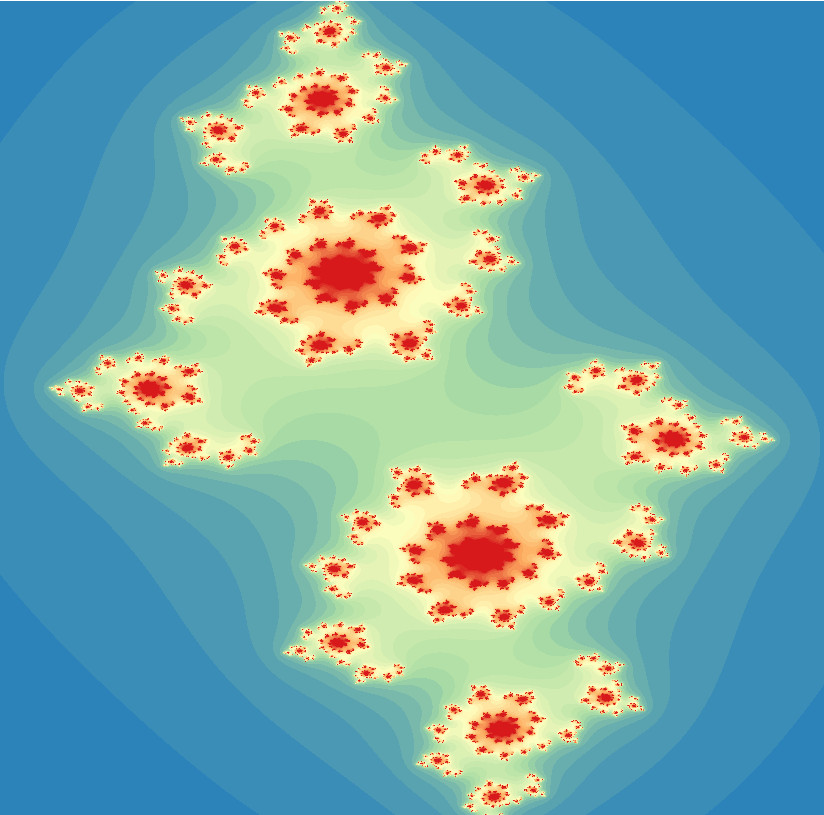
\includegraphics[scale=0.2]{./images/fractal16k16k}
\end{figure}
 
}

\frame{\frametitle{Julia Set - multi-GPU speedup} 
	\begin{figure}
	\centering
	\includegraphics[width=0.55\textwidth]{images/fractal_false_scaling}
	\caption{Julia set speedups obtained on single-GPU execution (K40 ,GTX980) and	multi-GPU execution on two devices ($144 \times 10^6$ grid points).}
\end{figure}
}

\frame{\frametitle{Julia Set - K40 vs GTX980} 
	\begin{figure}
		\centering
		\includegraphics[width=1\textwidth]{images/fractal12k_k40_980_true}
		\caption{Time and Speed-up for the Julia Set case ($1200 \times 10^6$ grid points) on two different GPUs: 1
			GTX980 and 1 K40 . The bottom and top horizontal axes indicate the amount of rows assigned to the K40 and GTX980 , respectively. .}
	\end{figure}
}


\subsection{Convolutional Filtering}
\frame{\frametitle{Convolutional Filtering} 
	\begin{itemize}
		\item Very common in image processing 
		\item The value of the grid point is substituted with a weighted average of neighboring points
		\item Little floating-point computation involved $\Longrightarrow$ memory bound
\end{itemize}
\begin{figure}
	\centering
	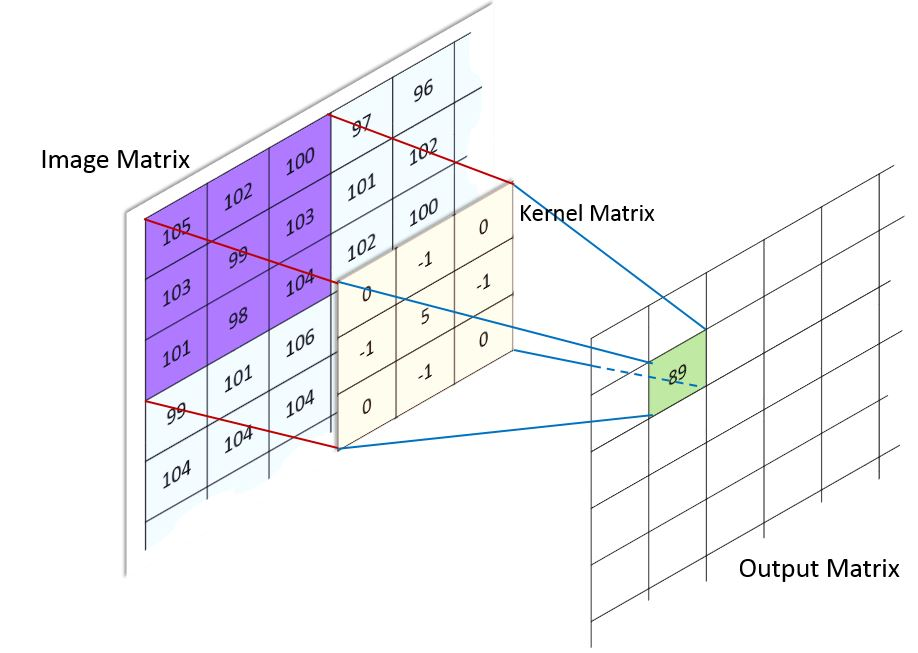
\includegraphics[scale=0.35]{./images/1}
\end{figure}

}

